


\begin{figure}[t]%h!
    \centering
    \begin{subfigure}{.47\textwidth}
        \centering
        %\includegraphics[width=0.9\linewidth]{spec_no_shift.jpg}
        %* Figure 1
        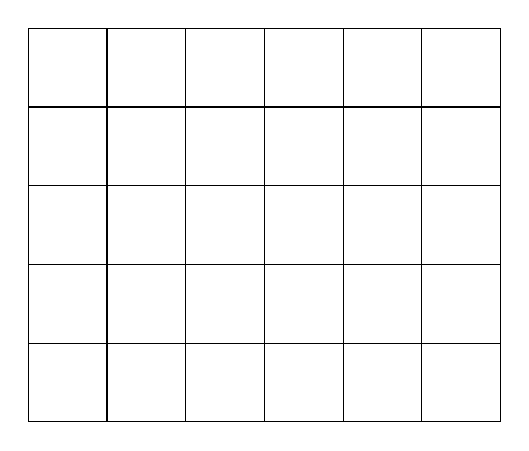
\begin{tikzpicture}[scale=1]
            % Define the tile
            \def\tile{
              % Draw the unit square
              \draw (0,0) rectangle (1,1);
            }
          
            % Draw the tiling pattern
            \foreach \x in {0,1,2,3,4,5}{
              \foreach \y in {0,1,2,3,4}{
                \pgfmathsetmacro{\shiftX}{\x} % Set horizontal shift
                \pgfmathsetmacro{\shiftY}{\y} % Set vertical shift
                \begin{scope}[shift={(\shiftX,\shiftY)}]
                  \tile % Draw the tile
                \end{scope}
              }
            }
        \end{tikzpicture}
        %* —————————————————
        \caption{Lattice tiling}
        \label{fig:lattice_tiling}
    \end{subfigure}\quad
    \begin{subfigure}{.47\textwidth}
        \centering
        %\includegraphics[width=0.9\linewidth]{spec_single_shift.jpg}
        %* Figure 2
        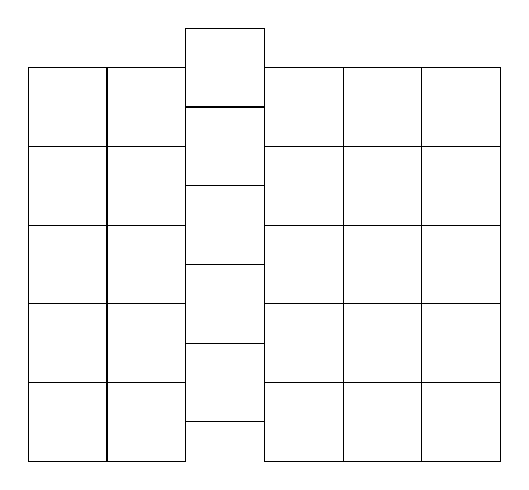
\begin{tikzpicture}[scale=1]
            % Define the tile
            \def\tile{
            % Draw the unit square
            \draw (0,0) rectangle (1,1);
            }
            \def\BetaSingle{0.5}
          
            % Draw the tiling pattern
            \foreach \x in {0,1,2,3,4,5}{
            \foreach \y in {0,1,2,3,4}{
                \ifnum\x=2 % Set vertical shift for the third column only
                    \pgfmathsetmacro{\shiftX}{\x} % No vertical shift for other columns
                    \pgfmathsetmacro{\shiftY}{\y + \BetaSingle} % Shift one unit upward
                \else
                    \pgfmathsetmacro{\shiftX}{\x} % No vertical shift for other columns
                    \pgfmathsetmacro{\shiftY}{\y} % No vertical shift
                \fi
                \begin{scope}[shift={(\shiftX,\shiftY)}]
                \tile % Draw the tile
                \end{scope}
            }}
        \end{tikzpicture}
        %* —————————————————
        \caption{Single shift vertical}
        \label{fig:single_shift_vertical_tiling}
    \end{subfigure}\\
    \begin{subfigure}{.47\textwidth}
        \centering
        %\includegraphics[width=0.9\linewidth]{multiple_shift_left_zero.jpg}
        %* Figure 3
        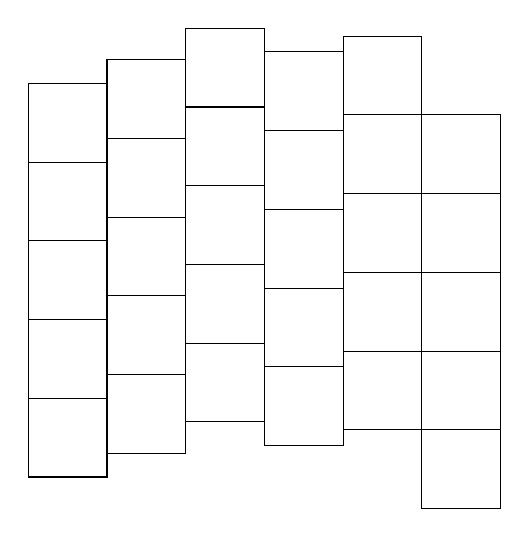
\begin{tikzpicture}
            % Define the tile
            \def\tile{
            % Draw the unit square
            \draw (0,0) rectangle (1,1);
            }

            % Shift list
            \def\BetaMinOne{0}
            \def\BetaZero{0.3}
            \def\BetaOne{0.7}
            \def\BetaTwo{0.4}
            \def\BetaThree{0.6}
            \def\BetaFour{-0.4}
            
            % Draw the tiling pattern
            \foreach \x in {0,1,2,3,4,5}{
            \foreach \y in {0,1,2,3,4}{
                \ifnum\x=0 % Set vertical shift for the third column only
                    \pgfmathsetmacro{\shiftX}{\x} % No vertical shift for other columns
                    \pgfmathsetmacro{\shiftY}{\y + \BetaMinOne} % Shift one unit upward
                \fi
                \ifnum\x=1
                    \pgfmathsetmacro{\shiftX}{\x}
                    \pgfmathsetmacro{\shiftY}{\y + \BetaZero}
                \fi
                \ifnum\x=2
                    \pgfmathsetmacro{\shiftX}{\x} 
                    \pgfmathsetmacro{\shiftY}{\y + \BetaOne} 
                \fi
                \ifnum\x=3
                    \pgfmathsetmacro{\shiftX}{\x}
                    \pgfmathsetmacro{\shiftY}{\y + \BetaTwo}
                \fi
                \ifnum\x=4
                    \pgfmathsetmacro{\shiftX}{\x}
                    \pgfmathsetmacro{\shiftY}{\y + \BetaThree}
                \fi
                \ifnum\x=5
                    \pgfmathsetmacro{\shiftX}{\x}
                    \pgfmathsetmacro{\shiftY}{\y + \BetaFour}
                \fi
                \begin{scope}[shift={(\shiftX,\shiftY)}]
                \tile % Draw the tile
                \end{scope}
            }}
        \end{tikzpicture}
        %* —————————————————
        \caption{Multiple shifts vertical}
        \label{fig:multiple_shift_vertical_tiling}
    \end{subfigure}\quad
    \begin{subfigure}{.47\textwidth}
        \centering
        %\includegraphics[width=0.9\linewidth]{multiple_shift_left_zero_horizontal.jpg}
        %* Figure 4
        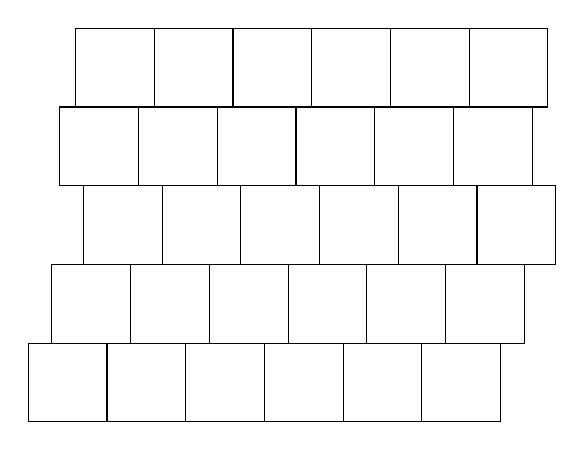
\begin{tikzpicture}
            % Define the tile
            \def\tile{
            % Draw the unit square
            \draw (0,0) rectangle (1,1);
            }

            % Shift list
            \def\BetaMinOne{0}
            \def\BetaZero{0.3}
            \def\BetaOne{0.7}
            \def\BetaTwo{0.4}
            \def\BetaThree{0.6}
            \def\BetaFour{-0.4}
            
            % Draw the tiling pattern
            \foreach \x in {0,1,2,3,4,5}{
            \foreach \y in {0,1,2,3,4}{
                \ifnum\y=0
                    \pgfmathsetmacro{\shiftX}{\x + \BetaMinOne}
                    \pgfmathsetmacro{\shiftY}{\y}
                \fi
                \ifnum\y=1
                    \pgfmathsetmacro{\shiftX}{\x + \BetaZero}
                    \pgfmathsetmacro{\shiftY}{\y}
                \fi
                \ifnum\y=2
                    \pgfmathsetmacro{\shiftX}{\x + \BetaOne} 
                    \pgfmathsetmacro{\shiftY}{\y} 
                \fi
                \ifnum\y=3
                    \pgfmathsetmacro{\shiftX}{\x + \BetaTwo}
                    \pgfmathsetmacro{\shiftY}{\y}
                \fi
                \ifnum\y=4
                    \pgfmathsetmacro{\shiftX}{\x + \BetaThree}
                    \pgfmathsetmacro{\shiftY}{\y}
                \fi
                \begin{scope}[shift={(\shiftX,\shiftY)}]
                \tile % Draw the tile
                \end{scope}
            }}
        \end{tikzpicture}
        %* —————————————————
        \caption{Multiple shifts horizontal}
        \label{fig:multiple_shift_horizontal_tiling}
    \end{subfigure}
    \caption{Text}
    \label{fig:tiling_figures}
\end{figure}
